\chapter{METODOLOGIA}
\label{cap:metodologia}

Este capítulo descreve a metodologia e as técnicas que serão empregados na pesquisa e desenvolvimento do sistema proposto, destacando as tecnologias e dispositivos necessários.

\section{Visão geral do sistema proposto}

O Sistema de Identificação de Condutores baseado em Técnicas de Inteligência Computacional terá a função de efetuar a identificação do condutor que dirige o veículo e detectar possíveis situações de roubo e furto do mesmo. Para tal, a identificação será feita por meio do reconhecimento de certos padrões de direção característicos e cada condutor. Isto é possível através da coleta de dados provenientes do barramento de comunicação do veículo, por meio da interface OBD-II e coletados pelo dispositivo de leitura ELM327, que transmite via \textit{bluetooth} para o \textit{smartphone} a ele conectado, que também fornece dados referentes à dinâmica de direção.

Um aplicativo no sistema operacional móvel Android recolherá os dados e então se formará um banco de dados referentes ao condutor. Antes de submeter os dados no algoritmo de identificação, será efetuado um processamento e fusão destes dados, a fim de remover ruídos e possíveis \textit{outliars}, além de melhorar a extração de características pelo sistema. Feito isso, o algoritmo de identificação irá cadastrar o condutor (em um primeiro momento), treinando-o com as características do mesmo, ou identificando a autenticidade do condutor em questão. O aplicativo retornará o veredicto com relação ao condutor e tomará as medidas necessárias. A Figura~\ref{fig:flux} apresenta graficamente o sistema como um todo, e os passos até a identificação.

\begin{figure}[!htb]
\centering
\caption{Visão geral do Sistema de Identificação de Condutores baseado em Técnicas de Inteligência Computacional.} %legenda
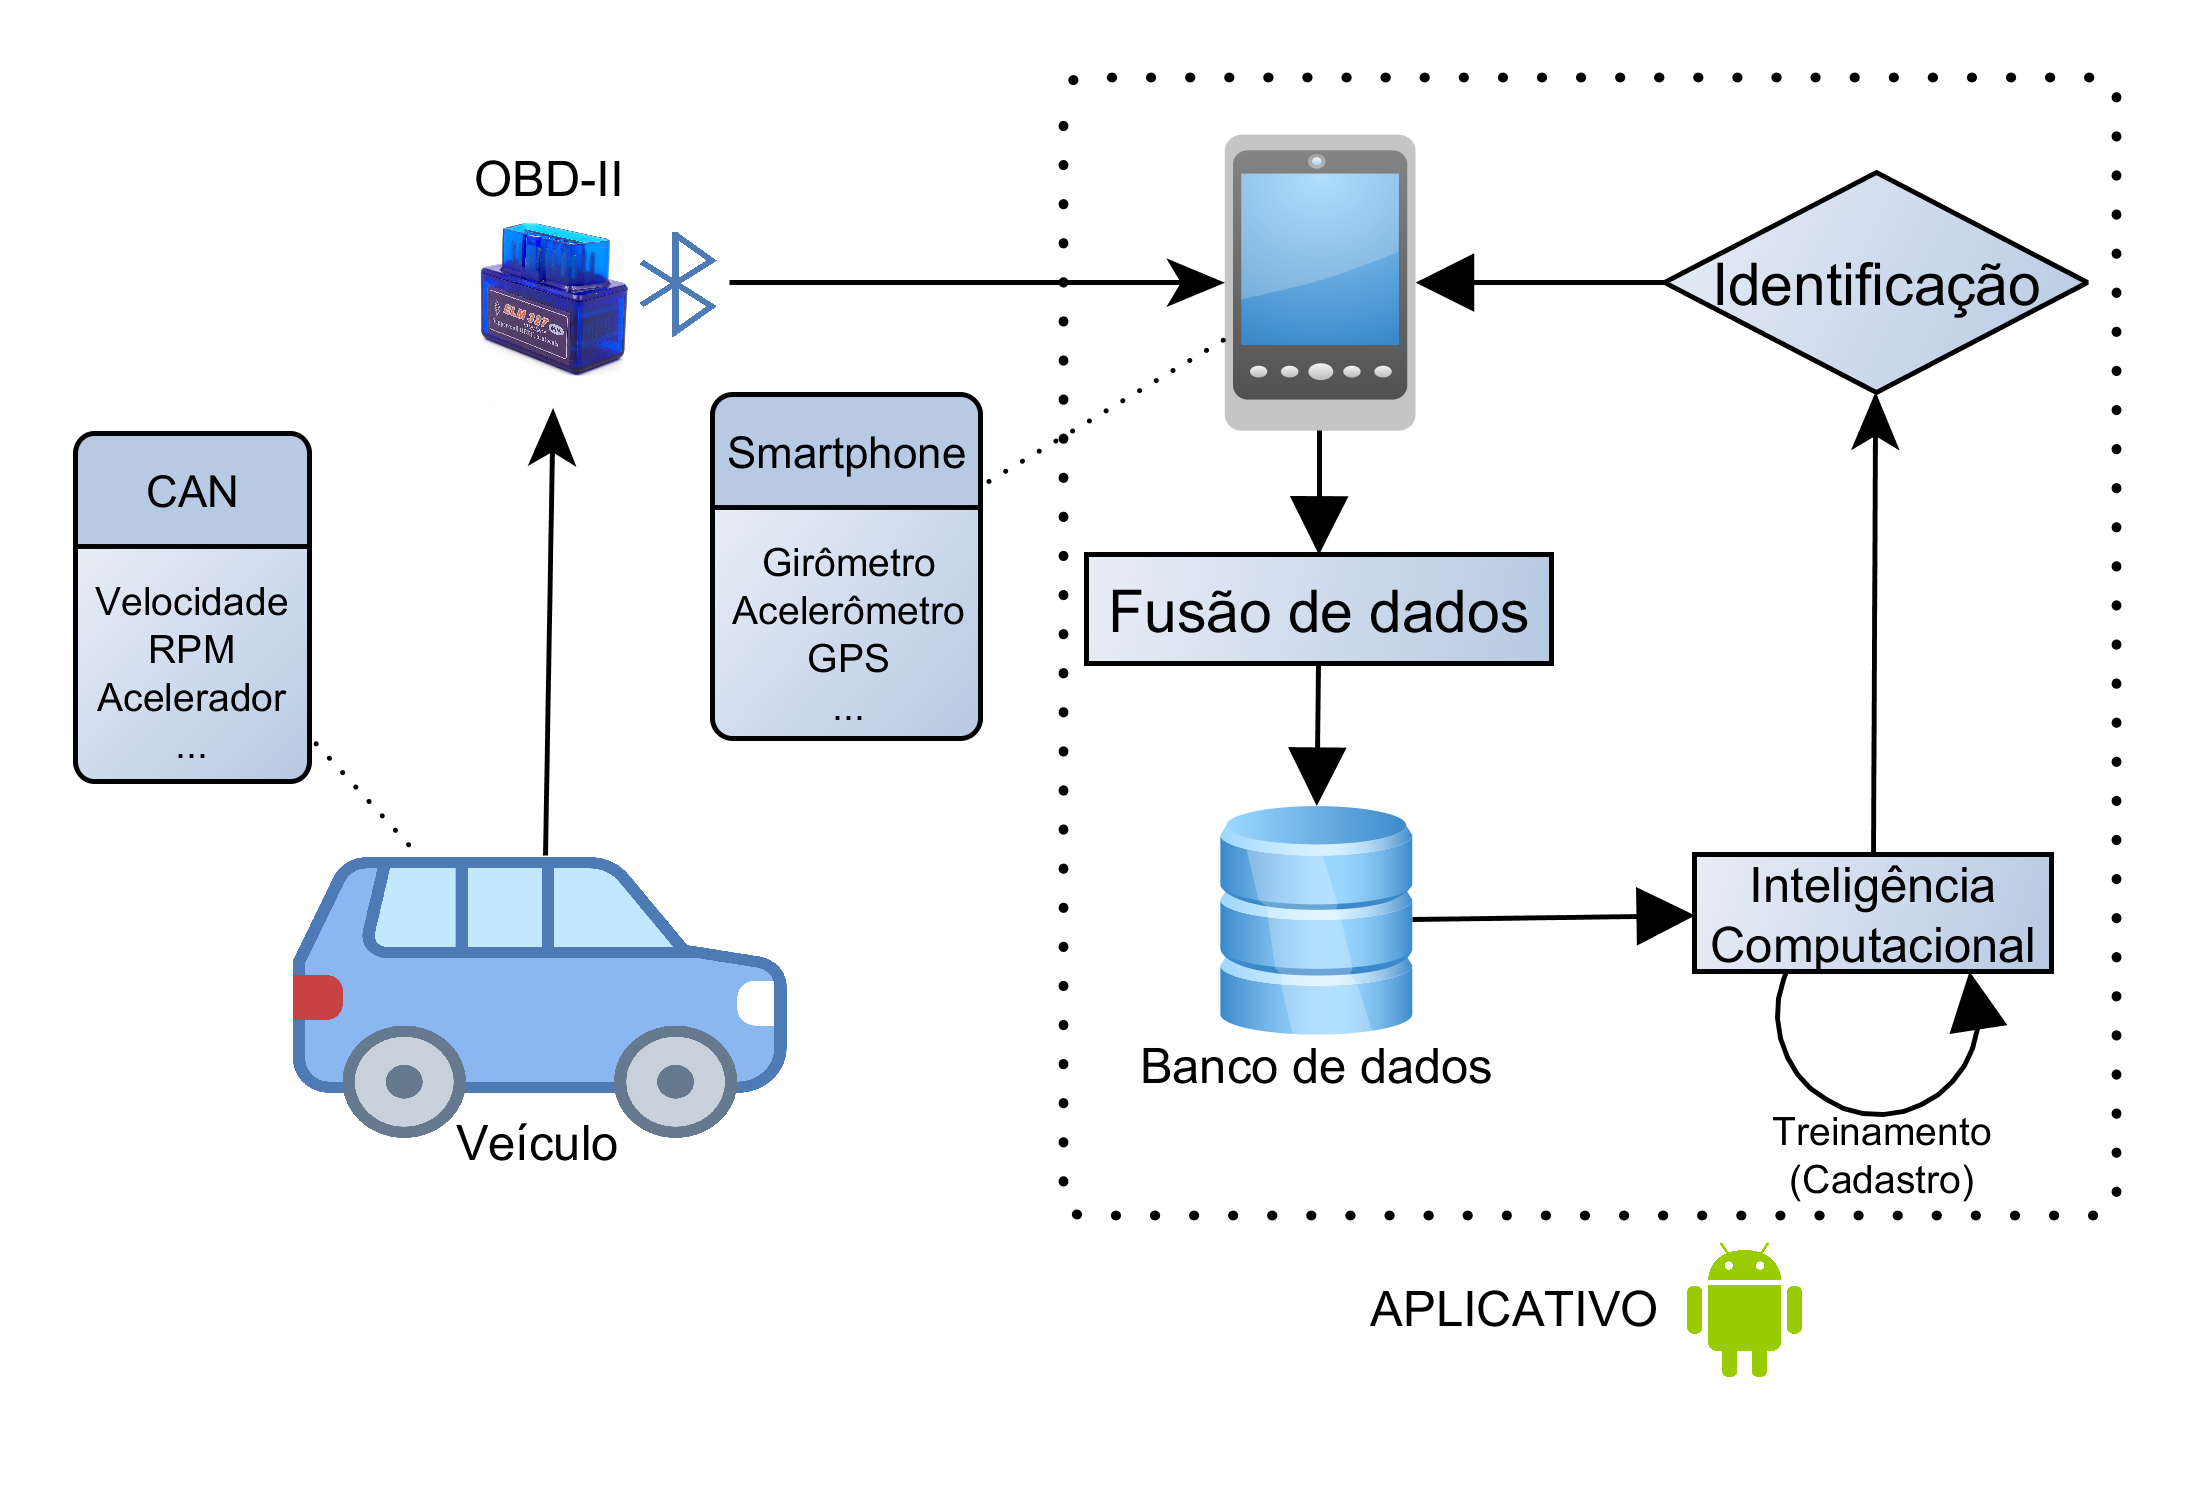
\includegraphics[scale=0.16]{FLUXOGRAMA.png}\\ 
{\small Fonte: Próprio autor.} %Fonte da imagem
\label{fig:flux} %rotulo para refencia
\end{figure}

\section{Desenvolvimento preliminar}

Para o desenvolvimento inicial do sistema proposto, será utilizado o \textit{dataset} UYANIK, cordialmente cedido pelo VPALAB da Universidade de Sabanci (Istambul, Turquia) \cite{Abut2007}. Este \textit{dataset} contém dados de um grande número de condutores colhidos a partir de dados do barramento CAN, sensores inerciais e GPS e é amplamente utilizado em diversos trabalhos que envolvem identificação de condutores \cite{Martinez2016a} \cite{jafarnejad2017} \cite{DelCampo2014}. Estes dados servirão para avaliar a aptidão das técnicas de processamento de dados e de inteligência computacional, a fim de se determinar as que melhores se encaixam na tarefa de identificação e autenticação dos condutores.

Estes resultados obtidos serão comparados com resultados quando o sistema tem como entrada dados oriundos da interface OBD-II e sensores inerciais presentes nos \textit{smarphones}. Isto se dá uma vez que o \textit{dataset} UYANIK foi colhido por meio de equipamentos mais sofisticados, com uma amostragem maior e menos ruidosos se comparado às fontes que serão utilizadas na aplicação final. O impacto desta diferença será avaliado no desempenho do sistema.

\section{Coleta de dados}

Para o desenvolvimento do sistema proposto, inicialmente será efetuada a coleta de dados que servirão como base de dados para o restante do projeto. Estes dados serão oriundos de duas fontes, a interface OBD-II (veículo) e sensores inerciais, geoposicionamento e magnéticos presentes no \textit{smartphone}.

O termo OBD-II significa \textit{On-Board Diagnostics} de segunda geração. Trata-se de um sistema que, ligado à central eletrônica do carro, permite a leitura e transmissão de diversos tipos de dados, por meio de um dispositivo eletrônico baseado no microcontrolador ELM327, que se conecta diretamente no barramento de comunicação do veículo (normanlmente CAN-bus) efetua leituras de diversos parâmetros. De acordo com \citeonline{Abuali2016}, estas informações coletadas podem ser utilizados para análise de dados, interface com usuário e coleta de dados de sensores.

Existem diversos casos na literatura que fazem uso de dados provenientes de leituras do OBD-II. Nos trabalhos de \citeonline{Martinez2015}, \citeonline{Pan2017}, \citeonline{Blaszczyk2014}, entre outros, faz-se uso de dados coletados pelo OBD-II e aplicadas técnicas de aprendizado de máquina para reconhecimento de alguns parâmetros, como agressividade, sonolência, entre outros.

Cada vez mais estudos de modelagem de comportamento do condutor têm aliado ao uso de dados provenientes do OBD-II o uso de dados sensoriais originários de \textit{smartphones}. De acordo com \citeonline{Saiprasert2017}, a capacidade de multi-sensoriamento de smartphone disponíveis no mercado propicia a coleta de uma preciosa gama de dados brutos. Dados de acelerômetros fornecem uma visão do movimento longitudinal e lateral do celular, e consequentemente do veículo, enquanto o GPS nele embarcado pode fornecer dados de localização em termos de longitude e latitude.

Na literatura, \textit{smartphones} têm sido empregados como ferramenta de coleta e processamento de dados em vasta gama de aplicações em sistemas veiculares. \citeonline{Hong2014} desenvolveram uma plataforma de modelagem de estilos de direção baseando-se somente em dados de sensores de \textit{smartphones}. Neste caso, os autores justificam que sistemas sensoriais para tal modelagem são caros, enquanto a penetração de mercado de \textit{smartphones} está praticamente consolidada, tendo assim aplicações desta natureza acessibilidade a praticamente todos os condutores.

Ciente do potencial de aplicação destas duas fontes de dados para aplicação em modelagem e identificação de comportamento de condutores, pretende-se que o sistema faça a leitura do barramento CAN do veículo, baseado do aplicativo desenvolvido por \citeonline{Neto2016}. Para tal, será avaliado quais variáveis serão monitoras de acordo com a aptidão de cada uma delas em detectar padrões característicos do condutor. Como apresentado por \citeonline{jafarnejad2017}, alguns sinais têm representatividade na identificação de condutores, a saber:

\begin{itemize}
    \item Porcentagem do Pedal de Acelerador.
    
    \item Ângulo do Volante em graus.
    
    \item Velocidade do Veículo.
    
    \item Rotação do Motor (RPM).
    
    \item Taxa de Guinada (Yaw Rate).
    
\end{itemize}

Para veículos brasileiros, alguns destes sinais, como o ângulo do volante, podem não estar disponíveis no mesmo. Para tal, será investigado o impacto da inexistência destes no processo e outras variáveis serão avaliadas como possíveis substitutas, de modo que a taxa de acertos do condutor seja maximizada. Não existe, porém, na literatura um consenso de quais variáveis têm maior capacidade de definir padrões que podem ser importantes na identificação do condutor.

\section{Processamento de sinais}

Para a aplicação de dados em qualquer técnica de aprendizado de máquina, é imprescindível que os dados sejam submetidos à um tratamento prévio, de tal modo à remover quaisquer ruídos, erros de medição e outras irregularidades nas informações.

Alguns trabalhados adotaram somente um processamento estatístico básico, como o cálculo de média acumulada, desvio padrão e amplitude dos dados, como visto em \citeonline{Carmona2015}. Por outro lado, o trabalho desenvolvido por \citeonline{Kumtepe2016} representa os sinais em forma de funções de densidade de probabilidade e então modelaram-nos por meio de Modelo de Misturas Gaussianas (GMM). Formam-se histogramas dos dados que ainda são filtrados por meio do método das médias móveis. Segundo o autor, este método proporciona uma representação efetiva de dados de direção.

Uma técnica de processamento de dados explorada por \citeonline{DelCampo2014}, especialmente para a aplicação de identificação de condutores, é a análise cepstral, aplicada como filtro e extrator de características. A técnica também é explora para processamento de sinais para identificação de condutores por \citeonline{jafarnejad2017}, em paralelo com extração estatística de características (média, mediana, curtoses, assimetria). Ambos trabalhos ressaltam que a análise cepstral é uma técnica com potencial para aplicação em identificação de condutores, por ser leve computacionalmente e adequada para futuras implementações em sistemas embarcados. Para tanto, pretende-se avaliar técnicas de pré-processamento de dados de forma a maximizar o desempenho do sistema \cite{Ahmadi-Pour2017}.



\section{Algoritmo de Identificação de Condutores}

Após a coleta dos dados referentes à dinâmica de direção e o processamento destes com o propósito de maximizar a extração de características, chega-se à fase de identificação do condutor por meio destes dados. Isto se dará por meio do uso de técnicas de aprendizado de máquina, em forma de classificador. Este processo será dividido em duas fases: primeiramente deve-se cadastrar o condutor autorizado à utilizar o veículo, por meio do treinamento do algoritmo. Na segunda fase, com o algoritmo já treinado para um ou mais condutores autorizados, deve-se avaliar e identificar o condutor que opera o veículo no momento.

O desenvolvimento desta parte do sistema passará inicialmente pela avaliação da técnica de aprendizado de máquina mais adequada para realizar a tarefa de identificação. Para tanto, alguns requisitos serão observados:

\begin{itemize}

    \item \textbf{Taxa de acertos:} este parâmetro consiste em avaliar qual técnica tem melhor aptidão em identificar a autenticidade do condutor, sem que o mesmo seja avaliado como sendo autorizado quando não o é e vice-versa. Este é um ponto crítico o sistema, pois em aplicações reais é imprescindível que o algoritmo não cometa equívocos quanto à decisão.
    
    \item \textbf{Custo computacional:} tendo em vista que o \textit{hardware} a ser utilizado é limitado (\textit{smartphone}, sistemas embarcados, FPGA, entre outros), o custo computacional da técnica deve ser cuidadosamente avaliado. O tempo de treinamento do algoritmo (cadastro) é um dos principais pontos a serem avaliados neste parâmetro, pois o mesmo deve ser rápido, mas ao mesmo tempo eficiente, com o propósito de não comprometer o desempenho do sistema.
    
    \item \textbf{Tempo de processamento:} tendo em vista que o sistema deverá verificar a autenticidade do condutor, o tempo em que o algoritmo leva para efetuar tal identificação é um ponto crucial, pois quanto mais rápido é identificado um intruso, maiores as chances de se impedir a ação criminosa.
    
\end{itemize}

No que diz respeito à \textit{driver behavior proffiling}, não existe uma unanimidade entre os autores em relação à qual técnica de aprendizado de máquina é a mais apropriada. Conforme apresentado por \citeonline{Meiring2015}, cada aplicação que envolva algum tipo de detecção de padrões (distração, sonolência, embriagues, agressividade) possui uma ou mais técnicas que tiveram resultados satisfatórios. Como existem poucos trabalhos na área de identificação de condutores, ainda se tem em aberto a possibilidade de testes em diversas técnicas de aprendizado de máquina, respeitando as premissas supracitadas.

Serão selecionados diversos algoritmos de classificação, dos quais serão avaliados o desempenho, de acordo com os requisitos definidos. Das técnicas que serão testadas, selecionou-se algumas que obtiveram desempenho satisfatório em outros trabalhos relacionados à identificação de condutores, dentre os quais pode-se citar:

\begin{itemize}
    \item \textbf{AdaBoost}, utilizado por \citeonline{jafarnejad2017}.
    
    \item \textbf{Gradient Boosting}, utilizado por \citeonline{jafarnejad2017}.
    
    \item \textbf{Extra Trees}, utilizado por \citeonline{jafarnejad2017}.
    
    \item \textbf{\textit{Extreme Learning Machines}}, utilizado por \citeonline{Martinez2016a}.
    
    
    \item \textbf{Máquinas de Vetor de Suporte}, utilizado por \citeonline{Chen2015} e \citeonline{jafarnejad2017}.
    
    \item \textbf{Redes Neurais Artificiais}, utilizado por \citeonline{DelCampo2014}.
    
    \item \textbf{Florestas Aleatórias}, utilizado por \citeonline{Wang2017a} e \citeonline{jafarnejad2017}.

\end{itemize}

É importante salientar que outros algoritmos ainda não utilizados em outros projetos poderão ser testados, uma vez identificada sua capacidade de desempenhar a tarefa de identificação e autenticação de condutores.

\section{Desenvolvimento de aplicação móvel Android}

Todos os elementos citados anteriormente irão compor um aplicativo para sistema operacional Android, que irá desempenhar a tarefa de identificação de condutores. Para isto, o desenvolvimento do mesmo irá se basear no trabalho desenvolvido por \citeonline{Neto2016}, que consiste basicamente num aplicativo que efetua leituras do dispositivo OBD-II, por meio da interface \textit{Bluetooth}, e também recolhe informações de sensores presentes no \textit{smartphone}, tais como acelerômetro, giroscópio, bússula (sensor de orientação) e GPS.

Diversos trabalhos exploram aplicações baseadas em Android, para a realização da tarefa de modelagem do perfil de condutores. Isto se deve muito à capacidade computacional que os \textit{smartphones} possuem atualmente, aliado aptidão que os sensores presentes nos mesmos têm de realizar leitura da dinâmica de direção como um todo.

Como exemplo, o aplicativo \textit{DrivingStyles} desenvolvido por \citeonline{Meseguer2017}, que por meio destas leituras, utiliza uma rede neural artificial treinada que identifica o estilo de direção do condutor entre calmo, normal e agressivo. De forma semelhante, \citeonline{Saiprasert2017} desenvolveram um aplicativo que monitora toda a dinâmica de direção e indica possíveis comportamentos que possam ser perigosos aos usuários do veículo.

Sendo assim, o uso de aplicativos móveis é uma ferramenta poderosa para implementação de sistemas que abranjam identificação de comportamento de condutores por meio de sensores que monitorem a dinâmica de direção como um todo. Portanto, para o presente trabalho, o desenvolvimento de um aplicativo que embarque todos os elementos que serão desenvolvidos é uma forma interessante de validar o sistema de uma forma simples, eficiente e acessível a um custo relativamente baixo.